\documentclass[11pt, a4paper]{article}

% ── Packages ────────────────────────────────────────────────
\usepackage[
  top=2.5cm, bottom=2.8cm,
  left=2.8cm, right=2.8cm
]{geometry}

\usepackage{fontenc}
\usepackage[utf8]{inputenc}
\usepackage{lmodern}
\usepackage{microtype}
\usepackage{parskip}
\usepackage{setspace}
\usepackage{titlesec}
\usepackage{titling}
\usepackage{fancyhdr}
\usepackage{booktabs}
\usepackage{array}
\usepackage{tabularx}
\usepackage{graphicx}
\usepackage{caption}
\usepackage{subcaption}
\usepackage{float}
\usepackage{xcolor}
\usepackage{hyperref}
\usepackage{amsmath}
\usepackage{amssymb}
\usepackage{listings}
\usepackage{enumitem}
\usepackage{mdframed}
\usepackage{tcolorbox}
\usepackage{etoolbox}

\tcbuselibrary{listings, skins, breakable}

% ── Colours ─────────────────────────────────────────────────
\definecolor{jpblue}{HTML}{003087}
\definecolor{jpgold}{HTML}{B5960A}
\definecolor{codebg}{HTML}{F7F8FA}
\definecolor{coderule}{HTML}{D0D4DC}
\definecolor{codecomment}{HTML}{6A737D}
\definecolor{codestring}{HTML}{032F62}
\definecolor{codekw}{HTML}{D73A49}
\definecolor{lightgray}{HTML}{F4F5F7}
\definecolor{rulecolor}{HTML}{C8CDD6}

% ── Hyperref setup ───────────────────────────────────────────
\hypersetup{
  colorlinks = true,
  linkcolor  = jpblue,
  citecolor  = jpblue,
  urlcolor   = jpblue,
  pdftitle   = {Stock Exchange Simulation — Programming Assignment},
}

% ── Typography ───────────────────────────────────────────────
\setstretch{1.15}

\titleformat{\section}
  {\large\bfseries\color{jpblue}}
  {\thesection.}{0.6em}{}
  [\vspace{-0.3em}\textcolor{rulecolor}{\rule{\linewidth}{0.4pt}}]

\titleformat{\subsection}
  {\normalsize\bfseries\color{jpblue!80}}
  {\thesubsection.}{0.5em}{}

\titleformat{\subsubsection}
  {\normalsize\itshape}
  {\thesubsubsection.}{0.5em}{}

\titlespacing*{\section}{0pt}{1.4em}{0.6em}
\titlespacing*{\subsection}{0pt}{1em}{0.4em}
\titlespacing*{\subsubsection}{0pt}{0.8em}{0.3em}

% ── Code listing style ───────────────────────────────────────
\lstdefinestyle{jpcode}{
  backgroundcolor   = \color{codebg},
  basicstyle        = \ttfamily\footnotesize,
  keywordstyle      = \color{codekw}\bfseries,
  stringstyle       = \color{codestring},
  commentstyle      = \color{codecomment}\itshape,
  numberstyle       = \tiny\color{gray},
  numbers           = left,
  numbersep         = 8pt,
  stepnumber        = 1,
  breaklines        = true,
  breakatwhitespace = false,
  showstringspaces  = false,
  frame             = single,
  framesep          = 4pt,
  rulecolor         = \color{coderule},
  xleftmargin       = 16pt,
  xrightmargin      = 4pt,
  tabsize           = 4,
  captionpos        = b,
}
\lstset{style=jpcode}

% tcolorbox wrapper for code files
\tcbset{
  codefile/.style={
    breakable,
    enhanced,
    colback      = codebg,
    colframe     = jpblue!40,
    fonttitle    = \bfseries\small\color{white},
    attach boxed title to top left = {yshift=-2mm, xshift=6mm},
    boxed title style = {
      colback    = jpblue,
      colframe   = jpblue,
      rounded corners,
      boxrule    = 0.4pt,
    },
    top          = 4mm,
    arc          = 3pt,
  }
}

% ── Page headers / footers ───────────────────────────────────
\pagestyle{fancy}
\fancyhf{}
\fancyhead[L]{\small\textcolor{jpblue}{\textbf{JPMorgan Chase} Quant Finance Mentorship Programme 2026}}
\fancyhead[R]{\small\textcolor{gray}{Programming Assignment}}
\fancyfoot[C]{\small\textcolor{gray}{\thepage}}
\renewcommand{\headrulewidth}{0.4pt}
\renewcommand{\headrule}{\hbox to\headwidth{\color{jpblue}\leaders\hrule height \headrulewidth\hfill}}
\renewcommand{\footrulewidth}{0pt}

% ── Utility: placeholder box ─────────────────────────────────
\newcommand{\graphplaceholder}[2][8cm]{%
  \begin{center}
  \begin{tikzpicture}
    \node[draw=rulecolor, fill=lightgray, rounded corners=4pt,
          minimum width=\linewidth, minimum height=#1,
          align=center, text=gray, font=\small\itshape] {#2};
  \end{tikzpicture}
  \end{center}
}

% ── Title block ──────────────────────────────────────────────
\renewcommand{\maketitle}{%
  \begin{center}
    {\footnotesize\scshape\color{gray} JPMorgan Chase Quant Finance Mentorship Programme 2026}\\[0.5em]
    {\LARGE\bfseries\color{jpblue} Stock Exchange Simulation}\\[0.3em]
    {\large Programming Assignment}\\[1.2em]
    \textcolor{rulecolor}{\rule{0.55\linewidth}{0.6pt}}\\[1.2em]
    \begin{tabular}{rl}
      \textbf{Team Name} & \texttt{[Team Name Here]} \\[0.4em]
      \textbf{Members}   & Farzana S [QMP37] \\
                         & Radha Gupta [QMP39] \\
                         & Khushi Goyal [QMP40] \\
                         & Vishakha Sinha [QMP41] \\
      \textbf{Date}      & \today \\
    \end{tabular}\\[1.4em]
    \textcolor{rulecolor}{\rule{0.55\linewidth}{0.6pt}}
  \end{center}
  \vspace{1.5em}
}

% ============================================================
\begin{document}

\maketitle
\thispagestyle{empty}

% ============================================================
\section{Introduction}

This project simulates a stock exchange environment, written in C++. The system models two parallel exchanges (Exchange A and Exchange B) trading five securities: AAPL, GOOGL, MSFT, AMZN, and META. Five regular traders place random buy and sell orders once per simulated second, while a sixth participant  (the Fast Trader) acts every half-second and looks for arbitrage opportunities between the two exchanges. All traders are managed through an Order Management System (OMS) that tracks their cash and stock holdings throughout the trading day.

% ============================================================
\section{System Design}

\subsection{Architecture Overview}

The system uses object-oriented C++. The main classes are \texttt{Exchange}, \texttt{OMS}, \texttt{Trader}, and \texttt{FastTrader}. Each trader owns an OMS, which holds references to both exchanges. The exchanges notify the OMS when a trade is filled or an order is cancelled, and the OMS updates the trader's cash and holdings accordingly. \texttt{FastTrader} inherits from \texttt{Trader} and overrides the \texttt{takeAction} method to run arbitrage logic instead of random trading.

\subsection{Core Components}

\subsubsection{Stock Exchange \& Order Book}

Each exchange maintains a separate order book per symbol. Bids are stored in a \texttt{std::map} sorted highest-first and asks sorted lowest-first, with each price level holding a \texttt{std::list} of orders to preserve time priority. When a new order arrives, the exchange checks trading hours, adds it to the book, attempts matching, and then prunes any price levels beyond the top five. At the end of the day, all remaining orders are cancelled.

\subsubsection{Order Management System (OMS)}

The OMS tracks a trader's cash balance and stock holdings in a map keyed by symbol. When \texttt{sendOrder} is called, it forwards the order to the correct exchange. The exchange then calls back \texttt{onOrderFulfilled} or \texttt{onOrderCancelled} to update balances. Portfolio value is calculated using the average last-traded price across both exchanges, falling back to \$10 if no trades have occurred yet.

\subsubsection{Trader}

Each regular trader, on every integer tick, iterates over all five symbols and randomly decides to buy or sell. The order price is picked randomly from the best bid, best ask, or mid-price. The trader prefers to send the order to whichever exchange does not already have an order at that price level, and falls back to a random choice if both or neither do. Before placing a buy order, the trader transfers funds from their bank account if the trading account balance is insufficient.

\subsubsection{Fast Trader}

The Fast Trader overrides \texttt{takeAction} and only runs \texttt{executeArbitrage} for each symbol. It checks if the best bid on one exchange is higher than the best ask on the other — if so, it simultaneously submits a buy order on the cheaper exchange and a sell order on the more expensive one, capped at 1000 shares. Both cash and existing holdings are checked before executing.

\subsubsection{Simulation Clock \& Event Loop}

The main loop steps forward in 0.5-second increments from time 0 to 23,400 (a 6.5-hour trading day). Regular traders fire at whole-number timestamps; the Fast Trader fires at half-second points (i.e.\ when \texttt{currentTime * 2} is odd). After each tick, profit/loss snapshots for all traders are recorded to the \texttt{ProfitTracker}.

% ============================================================
\section{Implementation}

\subsection{Code Files}

The project is organised into the following source files.

% ── File 1 ──────────────────────────────────────────────────
\begin{tcolorbox}[codefile, title={\texttt{Common.h}}]
\begin{lstlisting}[language=C++, numbers=none, caption={}]

#pragma once
#include <string>
#include <vector>
#include <memory>

enum class OrderSide
{
    BUY,
    SELL
};

struct Order
{
    long long orderId;
    int traderId;
    std::string symbol;
    OrderSide side;
    double price;
    int quantity;
    double timestamp;
};

struct Trade
{
    std::string symbol;
    double price;
    int quantity;
    double timestamp;
    int buyerId;
    int sellerId;
};

struct Quote
{
    double price;
    int quantity;
};

enum class CancellationReason
{
    OUTSIDE_TOP_5,
    END_OF_DAY,
    OUTSIDE_TRADING_HOURS
};

struct OrderCancellation
{
    Order order;
    CancellationReason reason;
    double timestamp;
};

\end{lstlisting}
\end{tcolorbox}

\vspace{0.6em}

\begin{tcolorbox}[codefile, title={\texttt{Exchange.h}}]
\begin{lstlisting}[language=C++, numbers=none, caption={}]

#pragma once
#include "Common.h"
#include <map>
#include <list>

class OMS;

class Exchange
{
public:
    Exchange(std::string name);

    // let an oms register itself with the exchange
    void registerOMS(int traderId, OMS *omsPtr);

    // indicates the last traded price of any security
    double getLastTradedPrice(const std::string &symbol) const;

    // indicates the current best bid and best offer
    std::pair<Quote, Quote> getBestBidOffer(const std::string &symbol) const;

    // indicates the top 5 bids and top 5 offers
    std::pair<std::vector<Quote>, std::vector<Quote>> getOrderBookDepth(const std::string &symbol) const;

    // accept bids or offers
    void acceptOrder(const Order &order);

    // trading hours management
    bool isTradingHours(double currentTime) const;
    void setTradingHours(double openTime, double closeTime);

    // end of day cleanup
    void endOfDayCleanup();

    // check if order exists at a specific price level for a symbol
    bool hasOrderAtPrice(const std::string &symbol, OrderSide side, double price) const;

    std::string getName() const;

private:
    std::string exchangeName;
    double marketOpenTime;
    double marketCloseTime;

    // map to link trader id to oms object
    std::map<int, OMS *> omsRegistry;

    // order matching engine
    // must follow price-time priority for all orders
    // implemented as a map of prices to a list of orders (for time priority)
    struct OrderBook
    {
        std::map<double, std::list<Order>, std::greater<double>> bids; // highest price first for bids
        std::map<double, std::list<Order>, std::less<double>> asks;    // lowest price first for asks
        double lastPrice = 0.0;

        // cached total quantity per price level
        // avoids O(n) loops on every quote read
        std::map<double, int, std::greater<double>> bidQty;
        std::map<double, int, std::less<double>> askQty;
    };

    std::map<std::string, OrderBook> symbolBooks;

    // order matching with price-time priority
    void match(const std::string &symbol);

    // cancel orders outside top 5
    void cancelOrdersOutsideTop5(const std::string &symbol);

    // cancel all pending orders for a symbol
    void cancelAllOrders(const std::string &symbol, CancellationReason reason);

    // notify OMS about trade
    void notifyTradeFulfilled(const Trade &trade);

    // notify OMS about order cancellation
    void notifyOrderCancelled(const OrderCancellation &cancellation);
};

\end{lstlisting}
\end{tcolorbox}

\vspace{0.6em}

\begin{tcolorbox}[codefile, title={\texttt{Exchange.cpp}}]
\begin{lstlisting}[language=C++, numbers=none, caption={}]

#include "Exchange.h"
#include "OMS.h"
#include <iostream>
#include <algorithm>

// Constructor
// Set default starting times to zero
Exchange::Exchange(std::string name) : exchangeName(std::move(name)), marketOpenTime(0.0), marketCloseTime(0.0)
{
}

// Connect a specific trader id to an OMS instance
void Exchange::registerOMS(int traderId, OMS *omsPtr)
{
    omsRegistry[traderId] = omsPtr;
}

// Look up a stock symbol and return the price at which the last trade occurred
double Exchange::getLastTradedPrice(const std::string &symbol) const
{
    auto it = symbolBooks.find(symbol);
    if (it != symbolBooks.end())
    {
        return it->second.lastPrice;
    }
    return 0.0;
}

// Return the top of the book
// The best available buy price and sell price for a symbol
std::pair<Quote, Quote> Exchange::getBestBidOffer(const std::string &symbol) const
{
    Quote bestBid = {0.0, 0};
    Quote bestAsk = {0.0, 0};

    auto it = symbolBooks.find(symbol);
    if (it != symbolBooks.end())
    {
        const auto &book = it->second;

        if (!book.bids.empty())
        {
            double price = book.bids.begin()->first;
            bestBid = {price, book.bidQty.at(price)};
        }

        if (!book.asks.empty())
        {
            double price = book.asks.begin()->first;
            bestAsk = {price, book.askQty.at(price)};
        }
    }

    return {bestBid, bestAsk};
}

std::pair<std::vector<Quote>, std::vector<Quote>> Exchange::getOrderBookDepth(const std::string &symbol) const
{
    std::vector<Quote> bidDepth;
    std::vector<Quote> askDepth;

    auto it = symbolBooks.find(symbol);
    if (it != symbolBooks.end())
    {
        const auto &book = it->second;

        // top 5 bids
        int count = 0;
        for (auto bidIt = book.bids.begin(); bidIt != book.bids.end() && count < 5; ++bidIt)
        {
            bidDepth.push_back({bidIt->first, book.bidQty.at(bidIt->first)});
            count++;
        }

        // top 5 asks
        count = 0;
        for (auto askIt = book.asks.begin(); askIt != book.asks.end() && count < 5; ++askIt)
        {
            askDepth.push_back({askIt->first, book.askQty.at(askIt->first)});
            count++;
        }
    }

    return {bidDepth, askDepth};
}

void Exchange::acceptOrder(const Order &order)
{
    // check trading hours
    if (!isTradingHours(order.timestamp))
    {
        OrderCancellation cancellation;
        cancellation.order = order;
        cancellation.reason = CancellationReason::OUTSIDE_TRADING_HOURS;
        cancellation.timestamp = order.timestamp;
        notifyOrderCancelled(cancellation);
        return;
    }

    // add order to the appropriate book
    OrderBook &book = symbolBooks[order.symbol];
    if (order.side == OrderSide::BUY)
    {
        book.bids[order.price].push_back(order);
        book.bidQty[order.price] += order.quantity;
    }
    else
    {
        book.asks[order.price].push_back(order);
        book.askQty[order.price] += order.quantity;
    }

    // attempt to match orders
    match(order.symbol);

    // after matching, ensure we only keep top 5 price levels
    cancelOrdersOutsideTop5(order.symbol);
}

bool Exchange::isTradingHours(double currentTime) const
{
    return currentTime >= marketOpenTime && currentTime <= marketCloseTime;
}

void Exchange::setTradingHours(double openTime, double closeTime)
{
    marketOpenTime = openTime;
    marketCloseTime = closeTime;
}

void Exchange::endOfDayCleanup()
{
    for (auto &pair : symbolBooks)
    {
        cancelAllOrders(pair.first, CancellationReason::END_OF_DAY);
    }
}

bool Exchange::hasOrderAtPrice(const std::string &symbol, OrderSide side, double price) const
{
    auto it = symbolBooks.find(symbol);
    if (it == symbolBooks.end())
    {
        return false;
    }

    const auto &book = it->second;
    if (side == OrderSide::BUY)
    {
        return book.bids.find(price) != book.bids.end();
    }
    else
    {
        return book.asks.find(price) != book.asks.end();
    }
}

std::string Exchange::getName() const
{
    return exchangeName;
}

// Price-Time Priority
void Exchange::match(const std::string &symbol)
{
    auto it = symbolBooks.find(symbol);
    if (it == symbolBooks.end())
        return;

    OrderBook &book = it->second;

    while (!book.bids.empty() && !book.asks.empty())
    {
        // Get the highest bid (bids sorted descending, so begin() = best/highest)
        auto bestBidIt = book.bids.begin();
        // Get the lowest ask (asks sorted ascending, so begin() = best/lowest)
        auto bestAskIt = book.asks.begin();

        double bidPrice = bestBidIt->first;
        double askPrice = bestAskIt->first;

        // check if there is a match (bid price >= ask price)
        if (bidPrice >= askPrice)
        {
            // get the orders at the front of the list (time priority)
            std::list<Order> &bidOrders = bestBidIt->second;
            std::list<Order> &askOrders = bestAskIt->second;

            if (bidOrders.empty() || askOrders.empty())
            {
                // safety check
                if (bidOrders.empty())
                {
                    book.bids.erase(bestBidIt);
                    book.bidQty.erase(bidPrice);
                }
                if (askOrders.empty())
                {
                    book.asks.erase(bestAskIt);
                    book.askQty.erase(askPrice);
                }
                continue;
            }

            Order &bidOrder = bidOrders.front();
            Order &askOrder = askOrders.front();

            // determine execution price based on the older order
            double tradePrice;
            if (bidOrder.timestamp < askOrder.timestamp)
            {
                tradePrice = bidPrice;
            }
            else
            {
                tradePrice = askPrice;
            }

            // determine trade quantity
            int tradeQuantity = std::min(bidOrder.quantity, askOrder.quantity);

            // create trade record
            Trade trade;
            trade.symbol = symbol;
            trade.price = tradePrice;
            trade.quantity = tradeQuantity;
            trade.timestamp = std::max(bidOrder.timestamp, askOrder.timestamp); // trade happens at the time of the newer order
            trade.buyerId = bidOrder.traderId;
            trade.sellerId = askOrder.traderId;

            // notify oms
            notifyTradeFulfilled(trade);

            // updates last traded price
            book.lastPrice = tradePrice;

            // decrement cached quantities
            book.bidQty[bidPrice] -= tradeQuantity;
            book.askQty[askPrice] -= tradeQuantity;

            // update quantities or remove filled orders
            bidOrder.quantity -= tradeQuantity;
            askOrder.quantity -= tradeQuantity;

            if (bidOrder.quantity == 0)
            {
                bidOrders.pop_front();
                if (bidOrders.empty())
                {
                    book.bids.erase(bestBidIt);
                    book.bidQty.erase(bidPrice);
                }
            }

            if (askOrder.quantity == 0)
            {
                askOrders.pop_front();
                if (askOrders.empty())
                {
                    book.asks.erase(bestAskIt);
                    book.askQty.erase(askPrice);
                }
            }
            // std::cout << "TRADE executed: " << symbol << " Qty: " << tradeQuantity << " Price: " << tradePrice << " Time: " << trade.timestamp << std::endl;
        }
        else
        {
            // no more matches possible
            break;
        }
    }
}

void Exchange::cancelOrdersOutsideTop5(const std::string &symbol)
{
    auto it = symbolBooks.find(symbol);
    if (it == symbolBooks.end())
        return;

    OrderBook &book = it->second;

    // For bids, keep the 5 highest prices.
    // bids map is sorted descending (std::greater), so begin() = highest (best).
    // To discard the lowest (worst) price levels, remove from prev(end()).
    while (book.bids.size() > 5)
    {
        auto lowestBidIt = std::prev(book.bids.end());
        double price = lowestBidIt->first;

        for (const auto &order : lowestBidIt->second)
        {
            OrderCancellation cancellation;
            cancellation.order = order;
            cancellation.reason = CancellationReason::OUTSIDE_TOP_5;
            cancellation.timestamp = order.timestamp;
            notifyOrderCancelled(cancellation);
        }

        book.bidQty.erase(price);
        book.bids.erase(lowestBidIt);
    }

    // For asks, keep the 5 lowest prices
    // Since map is sorted ascending, the top asks are at the beginning
    // We remove from the end (highest prices)
    while (book.asks.size() > 5)
    {
        auto highestAskIt = std::prev(book.asks.end());
        double price = highestAskIt->first;

        for (const auto &order : highestAskIt->second)
        {
            OrderCancellation cancellation;
            cancellation.order = order;
            cancellation.reason = CancellationReason::OUTSIDE_TOP_5;
            cancellation.timestamp = order.timestamp;
            notifyOrderCancelled(cancellation);
        }

        book.askQty.erase(price);
        book.asks.erase(highestAskIt);
    }
}

void Exchange::cancelAllOrders(const std::string &symbol, CancellationReason reason)
{
    auto it = symbolBooks.find(symbol);
    if (it == symbolBooks.end())
        return;

    OrderBook &book = it->second;

    // cancel all bids
    // at the end of the day
    for (auto &pair : book.bids)
    {
        for (const auto &order : pair.second)
        {
            OrderCancellation cancellation;
            cancellation.order = order;
            cancellation.reason = reason;
            cancellation.timestamp = marketCloseTime;
            notifyOrderCancelled(cancellation);
        }
    }
    book.bids.clear();
    book.bidQty.clear();

    // cancel all asks
    for (auto &pair : book.asks)
    {
        for (const auto &order : pair.second)
        {
            OrderCancellation cancellation;
            cancellation.order = order;
            cancellation.reason = reason;
            cancellation.timestamp = marketCloseTime;
            notifyOrderCancelled(cancellation);
        }
    }
    book.asks.clear();
    book.askQty.clear();
}

void Exchange::notifyTradeFulfilled(const Trade &trade)
{
    // notify buyer
    if (omsRegistry.count(trade.buyerId))
    {
        omsRegistry[trade.buyerId]->onOrderFulfilled(trade);
    }

    // notify seller
    if (omsRegistry.count(trade.sellerId))
    {
        omsRegistry[trade.sellerId]->onOrderFulfilled(trade);
    }
}

void Exchange::notifyOrderCancelled(const OrderCancellation &cancellation)
{
    if (omsRegistry.count(cancellation.order.traderId))
    {
        omsRegistry[cancellation.order.traderId]->onOrderCancelled(cancellation);
    }
}

\end{lstlisting}
\end{tcolorbox}

\vspace{0.6em}

\begin{tcolorbox}[codefile, title={\texttt{OMS.h}}]
\begin{lstlisting}[language=C++, numbers=none, caption={}]

#pragma once
#include "Common.h"
#include "Exchange.h"
#include <map>

class OMS
{
public:
    OMS(int traderId, Exchange &exchA, Exchange &exchB);

    // track the trader's cash in the trading account
    double getCashBalance() const;

    // add and withdraw cash from the trading account
    void depositCash(double amount);
    void withdrawCash(double amount);

    // indicates the current value of the trader's portfolio (cash + stock holdings)
    double getPortfolioValue() const;

    // get holdings for a specific symbol
    int getHoldings(const std::string &symbol) const;

    // get all holdings
    const std::map<std::string, int> &getAllHoldings() const;

    // place buy or sell orders
    // 0 = exchangeA, 1 = exchangeB
    void sendOrder(const Order &order, int exchangeTarget);

    // callback for when exchange matches a trade
    void onOrderFulfilled(const Trade &trade);

    // callback for when exchange cancels an order
    void onOrderCancelled(const OrderCancellation &cancellation);

    // get references to exchanges for querying market data
    Exchange &getExchangeA();
    Exchange &getExchangeB();
    const Exchange &getExchangeA() const;
    const Exchange &getExchangeB() const;

    // initialize starting portfolio
    void initializePortfolio(double cash, const std::map<std::string, int> &initialHoldings);

private:
    int traderId;
    double cashBalance;

    // a map to track stocks
    // key: stock symbol
    // value: quantity of shares held
    std::map<std::string, int> holdings;

    // pending orders sent to exchange, key: orderId
    std::map<long long, Order> pendingOrders;

    // references to the two identical exchanges
    Exchange &exchangeA;
    Exchange &exchangeB;
};


\end{lstlisting}
\end{tcolorbox}

\vspace{0.6em}

\begin{tcolorbox}[codefile, title={\texttt{OMS.cpp}}]
\begin{lstlisting}[language=C++, numbers=none, caption={}]


#include "OMS.h"
#include <algorithm>
#include <iostream>

// Constructor
OMS::OMS(int traderId, Exchange &exchA, Exchange &exchB)
    : traderId(traderId), cashBalance(0.0), exchangeA(exchA), exchangeB(exchB)
{
}

double OMS::getCashBalance() const
{
    return cashBalance;
}

void OMS::depositCash(double amount)
{
    cashBalance += amount;
}

void OMS::withdrawCash(double amount)
{
    cashBalance -= amount;
}

// Calculate the total net worth of the trader
double OMS::getPortfolioValue() const
{
    double stockValue = 0.0;
    for (const auto &pair : holdings)
    {
        const std::string &sym = pair.first;
        int qty = pair.second;

        if (qty <= 0)
            continue;

        // use best available last traded price across both exchanges
        double priceA = exchangeA.getLastTradedPrice(sym);
        double priceB = exchangeB.getLastTradedPrice(sym);

        double refPrice = 10.0; // Fallback default

        // Use average if both have trades, otherwise use the one that has a price
        if (priceA > 0.0 && priceB > 0.0)
        {
            refPrice = (priceA + priceB) / 2.0;
        }
        else if (priceA > 0.0)
        {
            refPrice = priceA;
        }
        else if (priceB > 0.0)
        {
            refPrice = priceB;
        }

        stockValue += refPrice * qty;
    }
    return cashBalance + stockValue;
}

int OMS::getHoldings(const std::string &symbol) const
{
    auto it = holdings.find(symbol);
    if (it != holdings.end())
        return it->second;
    return 0;
}

const std::map<std::string, int> &OMS::getAllHoldings() const
{
    return holdings;
}

void OMS::sendOrder(const Order &order, int exchangeTarget)
{
    // track pending order
    pendingOrders[order.orderId] = order;

    if (exchangeTarget == 0)
        exchangeA.acceptOrder(order);
    else
        exchangeB.acceptOrder(order);
}

// Update the books after a trade happens
void OMS::onOrderFulfilled(const Trade &trade)
{
    double tradeValue = trade.price * trade.quantity;

    if (trade.buyerId == traderId)
    {
        // we bought: deduct cash, add shares
        cashBalance -= tradeValue;
        holdings[trade.symbol] += trade.quantity;

        // guard against floating point drift
        if (cashBalance < 0.0)
            cashBalance = 0.0;
    }
    else if (trade.sellerId == traderId)
    {
        // we sold: add cash, deduct shares
        cashBalance += tradeValue;
        holdings[trade.symbol] -= trade.quantity;

        // guard against over-selling
        if (holdings[trade.symbol] < 0)
            holdings[trade.symbol] = 0;
    }
}

void OMS::onOrderCancelled(const OrderCancellation &cancellation)
{
    // remove from pending orders tracking
    pendingOrders.erase(cancellation.order.orderId);
}

Exchange &OMS::getExchangeA()
{
    return exchangeA;
}

Exchange &OMS::getExchangeB()
{
    return exchangeB;
}

const Exchange &OMS::getExchangeA() const
{
    return exchangeA;
}

const Exchange &OMS::getExchangeB() const
{
    return exchangeB;
}

void OMS::initializePortfolio(double cash, const std::map<std::string, int> &initialHoldings)
{
    cashBalance = cash;
    holdings = initialHoldings;
}


\end{lstlisting}
\end{tcolorbox}

\vspace{0.6em}

\begin{tcolorbox}[codefile, title={\texttt{Trader.h}}]
\begin{lstlisting}[language=C++, numbers=none, caption={}]

#pragma once
#include "OMS.h"
#include <vector>
#include <random>

class Trader
{
public:
    Trader(int id, double initialBankBalance, std::shared_ptr<OMS> oms);
    virtual ~Trader() = default;

    // perform an action
    // called at integer times for regular traders
    virtual void takeAction(double currentTime);

    // initialize trader with random portfolio
    void initializePortfolio(const std::vector<std::string> &symbols);

    // deposit money from bank to trading account if needed
    void depositFromBank(double amount);

    // check if trader can continue trading
    bool canTrade() const;

    // get trader profit/loss at end of day
    double calculateProfitLoss(const std::vector<std::string> &symbols) const;

    int getId() const;

protected:
    int id;
    std::vector<std::string> tradedSymbols;
    // bank account with a fixed amount of balance
    double bankAccountBalance;
    // initial bank balance for profit calculation
    double initialBankBalance;
    // true initial total wealth (bank + cash + stocks at t=0), used as P&L baseline
    double initialTotalWealth;
    // access to order management system
    std::shared_ptr<OMS> oms;

    // random number generator for this trader
    std::mt19937 rng;

    // decide whether to buy or sell
    OrderSide decideBuyOrSell();

    // decide the price at which the buy or sell order is placed
    // randomizes between best bid, best ask, or mid-price
    double calculateOrderPrice(const std::string &symbol, OrderSide side);

    // select which exchange to send order to
    int selectExchange(const std::string &symbol, OrderSide side, double price);

    // get best bid/ask across both exchanges
    Quote getBestBid(const std::string &symbol) const;
    Quote getBestAsk(const std::string &symbol) const;

    // check if trader has sufficient funds/shares for order
    bool canPlaceOrder(const std::string &symbol, OrderSide side, double price, int quantity) const;

    // generate a unique incrementing order id
    static long long generateOrderId();
};


\end{lstlisting}
\end{tcolorbox}

\vspace{0.6em}

\begin{tcolorbox}[codefile, title={\texttt{Trader.cpp}}]
\begin{lstlisting}[language=C++, numbers=none, caption={}]

#include "Trader.h"
#include <iostream>
#include <algorithm>
#include <numeric>
#include <cmath>
#include <utility>

// Constructor
Trader::Trader(int id, double initialBankBalance, std::shared_ptr<OMS> oms)
    : id(id), bankAccountBalance(initialBankBalance), initialBankBalance(initialBankBalance), oms(std::move(oms))
{
    std::random_device rd;
    rng.seed(rd());
}

// Called every tick
void Trader::takeAction(double currentTime)
{
    for (const auto &symbol : tradedSymbols)
    {
        OrderSide side = decideBuyOrSell();

        // calculate price according to rules
        double price = calculateOrderPrice(symbol, side);
        int quantity = 1000;
        if (side == OrderSide::SELL && oms->getHoldings(symbol) < 1000 && oms->getHoldings(symbol) > 0)
        {
            quantity = oms->getHoldings(symbol);
        }

        // check feasibility and transfer funds if necessary
        if (canPlaceOrder(symbol, side, price, quantity))
        {
            if (side == OrderSide::BUY)
            {
                double cost = price * quantity;
                double currentCash = oms->getCashBalance();
                if (currentCash < cost)
                {
                    double deficit = cost - currentCash;

                    if (bankAccountBalance >= deficit)
                    {
                        depositFromBank(deficit);
                    }
                }
            }

            // recheck after potential deposit
            if (side == OrderSide::BUY)
            {
                if (oms->getCashBalance() < price * quantity)
                    continue;
            }

            int exchangeIndex = selectExchange(symbol, side, price); // 0 = A, 1 = B

            Order order;
            // generate a unique incrementing id
            order.orderId = generateOrderId();
            order.traderId = id;
            order.symbol = symbol;
            order.side = side;
            order.price = price;
            order.quantity = quantity;
            order.timestamp = currentTime;

            oms->sendOrder(order, exchangeIndex);
        }
    }
}

void Trader::initializePortfolio(const std::vector<std::string> &symbols)
{
    tradedSymbols = symbols;
    std::map<std::string, int> initialHoldings;
    // random initial stock
    std::uniform_int_distribution<> qtyDist(10000, 50000);

    for (const auto &sym : symbols)
    {
        initialHoldings[sym] = (qtyDist(rng) / 1000) * 1000;
    }

    // move half of bank balance to trading account initially
    double initialTradingCash = initialBankBalance * 0.5;
    if (bankAccountBalance >= initialTradingCash)
    {
        oms->initializePortfolio(initialTradingCash, initialHoldings);
        bankAccountBalance -= initialTradingCash;
    }
    else
    {
        oms->initializePortfolio(0.0, initialHoldings);
    }

    // record true starting wealth after free stocks are allocated
    // getPortfolioValue() includes both oms cash and stock holdings
    initialTotalWealth = bankAccountBalance + oms->getPortfolioValue();
}

void Trader::depositFromBank(double amount)
{
    if (bankAccountBalance >= amount)
    {
        bankAccountBalance -= amount;
        oms->depositCash(amount);
    }
}

bool Trader::canTrade() const
{
    // if they run out of money or stocks to sell, stop taking any actions
    bool haveStocks = false;
    for (const auto &pair : oms->getAllHoldings())
    {
        if (pair.second > 0)
        {
            haveStocks = true;
            break;
        }
    }

    // total cash
    double totalCash = bankAccountBalance + oms->getCashBalance();

    return (totalCash > 1.0) || haveStocks;
}

double Trader::calculateProfitLoss(const std::vector<std::string> &symbols) const
{
    // getPortfolioValue() already includes oms cash + stock value, so we only add bank balance
    double currentAssets = bankAccountBalance + oms->getPortfolioValue();
    return currentAssets - initialTotalWealth;
}

int Trader::getId() const
{
    return id;
}

OrderSide Trader::decideBuyOrSell()
{
    std::uniform_int_distribution<> dist(0, 1);
    return (dist(rng) == 0) ? OrderSide::BUY : OrderSide::SELL;
}

double Trader::calculateOrderPrice(const std::string &symbol, OrderSide side)
{
    Quote bestBid = getBestBid(symbol);
    Quote bestAsk = getBestAsk(symbol);

    bool hasBid = (bestBid.quantity > 0);
    bool hasAsk = (bestAsk.quantity > 0);

    // if no bids or offers present in the market
    if (!hasBid && !hasAsk)
    {
        // place arbitrarily 5% above or below last traded price.
        double lastPriceA = oms->getExchangeA().getLastTradedPrice(symbol);
        double lastPriceB = oms->getExchangeB().getLastTradedPrice(symbol);

        double refPrice = 0.0;
        if (lastPriceA > 0.0 && lastPriceB > 0.0)
        {
            refPrice = (lastPriceA + lastPriceB) / 2.0; // Use average
        }
        else
        {
            refPrice = std::max(lastPriceA, lastPriceB); // If one is 0, pick the other
        }

        if (refPrice <= 0.0001)
            refPrice = 10.0;

        std::uniform_int_distribution<> dist(0, 1);
        if (dist(rng) == 0)
            return refPrice * 1.05;
        else
            return refPrice * 0.95;
    }

    std::vector<double> options;
    if (hasBid)
        options.push_back(bestBid.price);
    if (hasAsk)
        options.push_back(bestAsk.price);
    if (hasBid && hasAsk)
        options.push_back((bestBid.price + bestAsk.price) / 2.0);

    // if some options are invalid, pick from valid ones.
    std::uniform_int_distribution<> dist(0, options.size() - 1);
    return options[dist(rng)];
}

int Trader::selectExchange(const std::string &symbol, OrderSide side, double price)
{
    bool existsInA = oms->getExchangeA().hasOrderAtPrice(symbol, side, price);
    bool existsInB = oms->getExchangeB().hasOrderAtPrice(symbol, side, price);

    if (existsInA && !existsInB)
        return 1; // Send to Exchange B
    if (existsInB && !existsInA)
        return 0; // Send to Exchange A

    // If exists in both or neither, choice is random
    std::uniform_int_distribution<> dist(0, 1);
    return dist(rng);
}

Quote Trader::getBestBid(const std::string &symbol) const
{
    auto resultA = oms->getExchangeA().getBestBidOffer(symbol);
    auto resultB = oms->getExchangeB().getBestBidOffer(symbol);

    Quote bidA = resultA.first;
    Quote bidB = resultB.first;

    if (bidA.quantity == 0 && bidB.quantity == 0)
        return {0.0, 0};
    if (bidA.quantity == 0)
        return bidB;
    if (bidB.quantity == 0)
        return bidA;

    // highest bid is best
    if (bidA.price > bidB.price)
        return bidA;
    if (bidB.price > bidA.price)
        return bidB;
    // tiebreaker
    return bidA;
}

Quote Trader::getBestAsk(const std::string &symbol) const
{
    auto resultA = oms->getExchangeA().getBestBidOffer(symbol);
    auto resultB = oms->getExchangeB().getBestBidOffer(symbol);

    Quote askA = resultA.second;
    Quote askB = resultB.second;

    if (askA.quantity == 0 && askB.quantity == 0)
        return {0.0, 0};
    if (askA.quantity == 0)
        return askB;
    if (askB.quantity == 0)
        return askA;

    // lowest ask is best
    if (askA.price < askB.price)
        return askA;
    if (askB.price < askA.price)
        return askB;
    // tiebreaker
    return askA;
}

bool Trader::canPlaceOrder(const std::string &symbol, OrderSide side, double price, int quantity) const
{
    if (side == OrderSide::BUY)
    {
        double cost = price * quantity;
        double currentTotal = oms->getCashBalance() + bankAccountBalance;
        return currentTotal >= cost;
    }
    else
    {
        return oms->getHoldings(symbol) >= quantity;
    }
}

long long Trader::generateOrderId()
{
    static long long counter = 0;
    return ++counter;
}

\end{lstlisting}
\end{tcolorbox}

\vspace{0.6em}

\begin{tcolorbox}[codefile, title={\texttt{FastTrader.h}}]
\begin{lstlisting}[language=C++, numbers=none, caption={}]

#pragma once
#include "Trader.h"

class FastTrader : public Trader
{
public:
    using Trader::Trader;

    // performs action at half-second intervals
    void takeAction(double currentTime) override;

private:
    // look for arbitrage opportunity and execute if possible
    // buy low at one exchange and sell high at another simultaneously
    void executeArbitrage(const std::string &symbol, double currentTime);
};

\end{lstlisting}
\end{tcolorbox}

\vspace{0.6em}

\begin{tcolorbox}[codefile, title={\texttt{FastTrader.cpp}}]
\begin{lstlisting}[language=C++, numbers=none, caption={}]

#include "FastTrader.h"
#include <algorithm>

void FastTrader::takeAction(double currentTime)
{
    for (const auto &symbol : tradedSymbols)
    {
        executeArbitrage(symbol, currentTime);
    }
}

void FastTrader::executeArbitrage(const std::string &symbol, double currentTime)
{
    auto [bidA, askA] = oms->getExchangeA().getBestBidOffer(symbol);
    auto [bidB, askB] = oms->getExchangeB().getBestBidOffer(symbol);

    // Case 1
    // Best bid on Exchange A > Best ask on Exchange B
    // Buy cheap on B, sell high on A
    if (bidA.quantity > 0 && askB.quantity > 0 && bidA.price > askB.price)
    {
        int qty = std::min({1000, bidA.quantity, askB.quantity});
        double cost = askB.price * qty;

        // need cash to buy and shares to sell simultaneously
        if (oms->getCashBalance() < cost)
            return;
        if (oms->getHoldings(symbol) < qty)
            return;

        Order buyOrder;
        buyOrder.orderId = generateOrderId();
        buyOrder.traderId = getId();
        buyOrder.symbol = symbol;
        buyOrder.side = OrderSide::BUY;
        buyOrder.price = askB.price; // buy at the ask on B
        buyOrder.quantity = qty;
        buyOrder.timestamp = currentTime;

        Order sellOrder;
        sellOrder.orderId = generateOrderId();
        sellOrder.traderId = getId();
        sellOrder.symbol = symbol;
        sellOrder.side = OrderSide::SELL;
        sellOrder.price = bidA.price; // sell at the bid on A
        sellOrder.quantity = qty;
        sellOrder.timestamp = currentTime;

        // buy on Exchange B
        oms->sendOrder(buyOrder, 1);
        // sell on Exchange A
        oms->sendOrder(sellOrder, 0);
    }

    // Case 2
    // Best bid on Exchange B > Best ask on Exchange A
    // Buy cheap on A, sell high on B
    else if (bidB.quantity > 0 && askA.quantity > 0 && bidB.price > askA.price)
    {
        int qty = std::min({1000, bidB.quantity, askA.quantity});
        double cost = askA.price * qty;

        if (oms->getCashBalance() < cost)
            return;
        if (oms->getHoldings(symbol) < qty)
            return;

        Order buyOrder;
        buyOrder.orderId = generateOrderId();
        buyOrder.traderId = getId();
        buyOrder.symbol = symbol;
        buyOrder.side = OrderSide::BUY;
        buyOrder.price = askA.price; // buy at the ask on A
        buyOrder.quantity = qty;
        buyOrder.timestamp = currentTime;

        Order sellOrder;
        sellOrder.orderId = generateOrderId();
        sellOrder.traderId = getId();
        sellOrder.symbol = symbol;
        sellOrder.side = OrderSide::SELL;
        sellOrder.price = bidB.price; // sell at the bid on B
        sellOrder.quantity = qty;
        sellOrder.timestamp = currentTime;

        // buy on Exchange A
        oms->sendOrder(buyOrder, 0);
        // sell on Exchange B
        oms->sendOrder(sellOrder, 1);
    }
}

\end{lstlisting}
\end{tcolorbox}

\vspace{0.6em}

\begin{tcolorbox}[codefile, title={\texttt{ProfitTracker.h}}]
\begin{lstlisting}[language=C++, numbers=none, caption={}]

#pragma once
#include <map>
#include <vector>
#include <string>

class ProfitTracker
{
public:
    void record(double time, int traderId, double profit);
    void exportCSV(const std::string &filename) const;

private:
    std::map<double, std::map<int, double>> data;
};

\end{lstlisting}
\end{tcolorbox}

\vspace{0.6em}

\begin{tcolorbox}[codefile, title={\texttt{ProfitTracker.cpp}}]
\begin{lstlisting}[language=C++, numbers=none, caption={}]

#include "ProfitTracker.h"
#include <fstream>
#include <set>

// Save a snapshot of the trader's profit at a given time
void ProfitTracker::record(double time, int traderId, double profit)
{
    data[time][traderId] = profit;
}

void ProfitTracker::exportCSV(const std::string &filename) const
{
    std::ofstream file(filename);

    std::set<int> traders;

    for (const auto &t : data)
    {
        for (const auto &p : t.second)
            traders.insert(p.first);
    }

    file << "time";
    for (const auto &trader : traders)
        file << "," << trader;
    file << "\n";

    for (const auto &t : data)
    {
        file << t.first;

        for (const auto &trader : traders)
        {
            auto it = t.second.find(trader);

            if (it != t.second.end())
                file << "," << it->second;
            else
                file << ",0";
        }

        file << "\n";
    }

    file.close();
}

\end{lstlisting}
\end{tcolorbox}

\vspace{0.6em}

\begin{tcolorbox}[codefile, title={\texttt{main.cpp}}]
\begin{lstlisting}[language=C++, numbers=none, caption={}]

#include "Exchange.h"
#include "Trader.h"
#include "FastTrader.h"
#include <vector>
#include <iostream>
#include <memory>
#include "ProfitTracker.h"

int main()
{
    // simulation parameters
    const double TIME_STEP = 0.5;
    const double TRADING_DAY_DURATION = 23400.0; // 6.5 hours
    const double MARKET_OPEN = 0.0;
    const double MARKET_CLOSE = TRADING_DAY_DURATION;

    // securities to trade
    std::vector<std::string> symbols = {"AAPL", "GOOGL", "MSFT", "AMZN", "META"};

    // create 2 identical stock exchanges
    Exchange exchangeA("EXCH_A");
    Exchange exchangeB("EXCH_B");

    // set trading hours for both exchanges
    exchangeA.setTradingHours(MARKET_OPEN, MARKET_CLOSE);
    exchangeB.setTradingHours(MARKET_OPEN, MARKET_CLOSE);

    // initialise traders with non-zero portfolios
    std::vector<std::unique_ptr<Trader>> traders;
    for (int i = 0; i < 5; ++i)
    {
        auto oms = std::make_shared<OMS>(i, exchangeA, exchangeB);

        // register OMS with exchanges
        exchangeA.registerOMS(i, oms.get());
        exchangeB.registerOMS(i, oms.get());

        // create trader with arbitrary bank balance
        auto trader = std::make_unique<Trader>(i, 100000000.0, oms);

        // initialise with random portfolio of stocks
        trader->initializePortfolio(symbols);

        traders.push_back(std::move(trader));
    }

    // initialise fast trader with non-zero portfolio
    auto fastOms = std::make_shared<OMS>(5, exchangeA, exchangeB);
    exchangeA.registerOMS(5, fastOms.get());
    exchangeB.registerOMS(5, fastOms.get());

    FastTrader fastTrader(5, 5000000.0, fastOms);
    fastTrader.initializePortfolio(symbols);
    ProfitTracker tracker;

    // simulation loop
    for (const auto &sym : symbols)
    {
        std::cout << sym << " ";
    }
    std::cout << "\n\n";

    for (double currentTime = 0.0; currentTime <= TRADING_DAY_DURATION; currentTime += TIME_STEP)
    {
        // regular traders take action at integer times
        if (static_cast<int>(currentTime) == currentTime)
        {
            for (auto &trader : traders)
            {
                if (trader->canTrade())
                {
                    trader->takeAction(currentTime);
                }
            }
        }

        // fast trader takes action at half-second points
        if (static_cast<int>(currentTime * 2) % 2 == 1)
        {
            if (fastTrader.canTrade())
            {
                fastTrader.takeAction(currentTime);
            }
        }

        for (auto &trader : traders)
        {
            double profit = trader->calculateProfitLoss(symbols);
            tracker.record(currentTime, trader->getId(), profit);
        }

        double fastProfit = fastTrader.calculateProfitLoss(symbols);
        tracker.record(currentTime, fastTrader.getId(), fastProfit);
    }

    // end of day cleanup
    // cancel all pending orders
    exchangeA.endOfDayCleanup();
    exchangeB.endOfDayCleanup();
    tracker.exportCSV("profits.csv");

    return 0;
}

\end{lstlisting}
\end{tcolorbox}

\vspace{0.6em}

% ============================================================
\section{Simulation Results}

The simulation was run four times with different random seeds to illustrate the
variability introduced by stochastic trader behaviour.  Initial conditions are
identical across runs: five regular traders and one Fast Trader, each seeded with
an arbitrary starting cash balance and a randomised non-zero portfolio across five
securities.  The trading day spans 6.5 hours (23{,}400 simulation steps of 0.5 s).

% ── Graph 1 ─────────────────────────────────────────────────
\subsection{Run 1}

\begin{figure}[H]
  \centering
  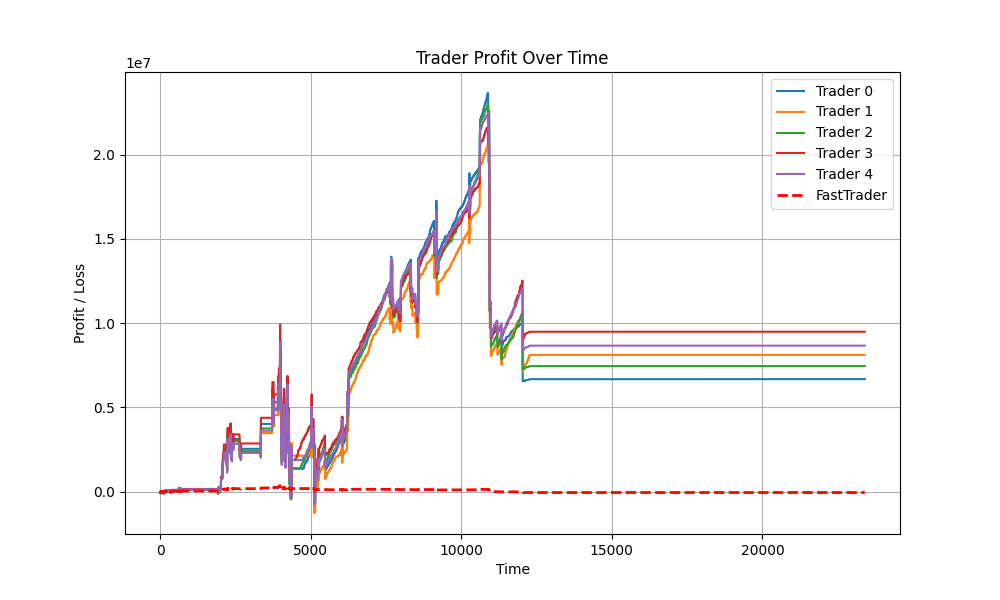
\includegraphics[width=\linewidth]{graphs/profit_graph_1.png}
  \caption{Cumulative P\&L per trader — Simulation Run 1.}
  \label{fig:run1}
\end{figure}

% ── Graph 2 ─────────────────────────────────────────────────
\subsection{Run 2}

\begin{figure}[H]
  \centering
  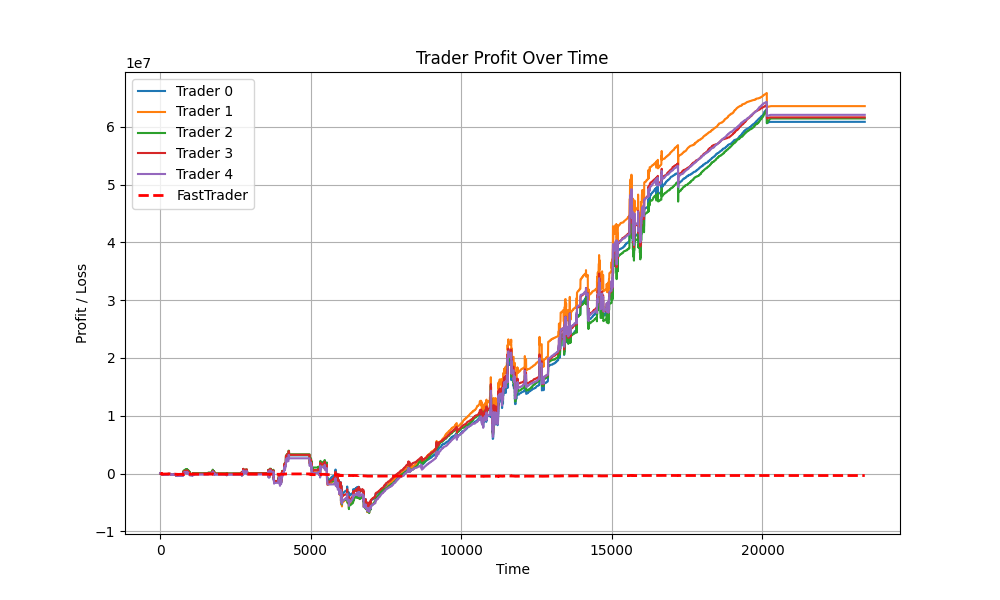
\includegraphics[width=\linewidth]{graphs/profit_graph_2.png}
  \caption{Cumulative P\&L per trader — Simulation Run 2.}
  \label{fig:run2}
\end{figure}

% ── Graph 3 ─────────────────────────────────────────────────
\subsection{Run 3}

\begin{figure}[H]
  \centering
  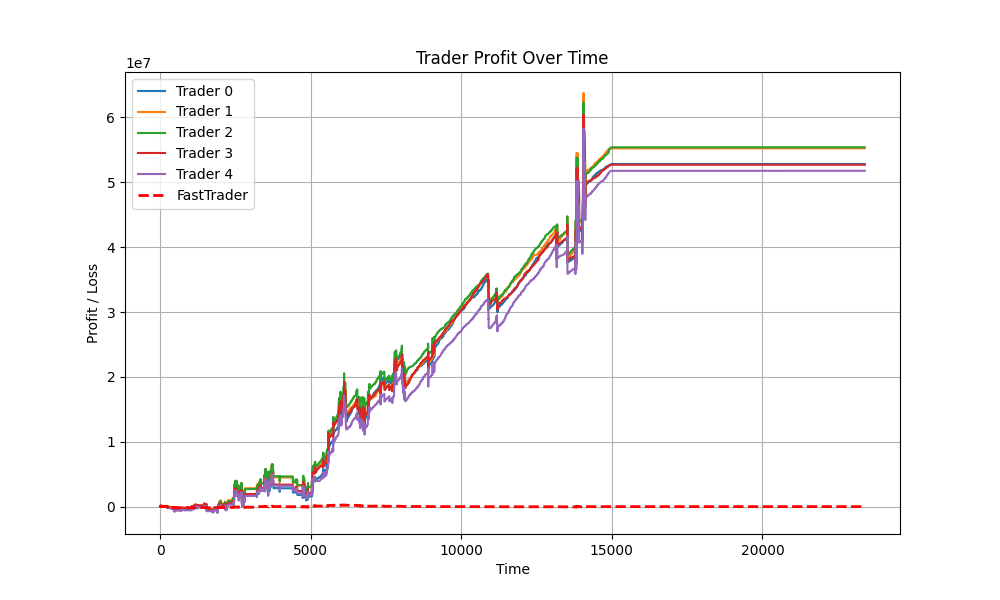
\includegraphics[width=\linewidth]{graphs/profit_graph_3.png}
  \caption{Cumulative P\&L per trader — Simulation Run 3.}
  \label{fig:run3}
\end{figure}

% ── Graph 4 ─────────────────────────────────────────────────
\subsection{Run 4}

\begin{figure}[H]
  \centering
  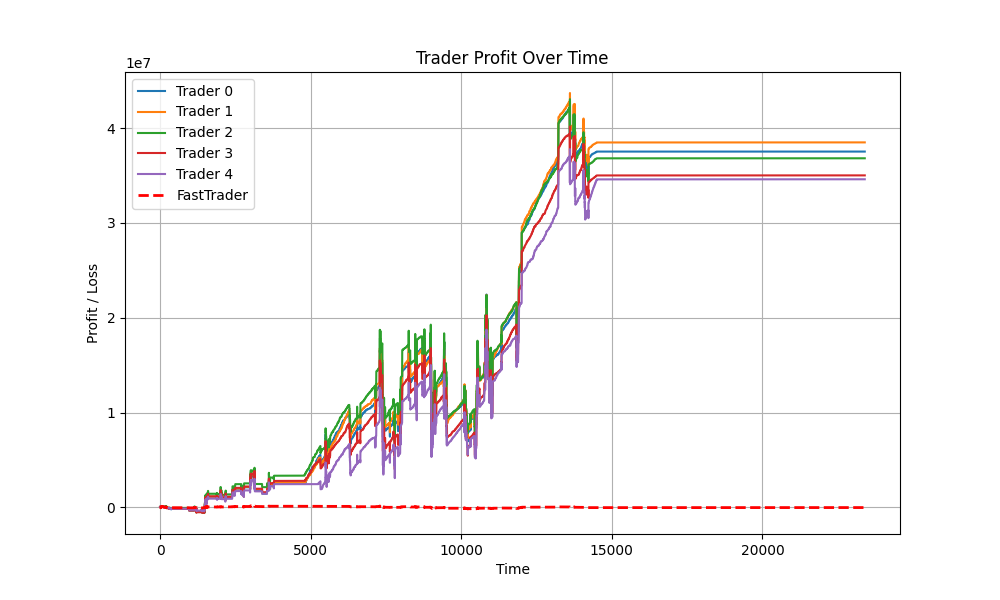
\includegraphics[width=\linewidth]{graphs/profit_graph_4.png}
  \caption{Cumulative P\&L per trader — Simulation Run 4.}
  \label{fig:run4}
\end{figure}

% ── Summary table ────────────────────────────────────────────
\subsection{End-of-Day Summary}

\begin{table}[H]
\centering
\caption{End-of-day profit / (loss) by participant across four simulation runs.
         Values in USD; parentheses denote losses.}
\label{tab:summary}
\small
\begin{tabularx}{\linewidth}{l*{4}{>{\centering\arraybackslash}X}}
\toprule
\textbf{Participant} & \textbf{Run 1} & \textbf{Run 2} & \textbf{Run 3} & \textbf{Run 4} \\
\midrule
Trader 1    & [+/- \$] & [+/- \$] & [+/- \$] & [+/- \$] \\
Trader 2    & [+/- \$] & [+/- \$] & [+/- \$] & [+/- \$] \\
Trader 3    & [+/- \$] & [+/- \$] & [+/- \$] & [+/- \$] \\
Trader 4    & [+/- \$] & [+/- \$] & [+/- \$] & [+/- \$] \\
Trader 5    & [+/- \$] & [+/- \$] & [+/- \$] & [+/- \$] \\
\midrule
Fast Trader & [+/- \$] & [+/- \$] & [+/- \$] & [+/- \$] \\
\bottomrule
\end{tabularx}
\end{table}

% ============================================================
\section{Analysis}

\subsection{Fast Trader Behaviour}

The Fast Trader checks every half-second whether the best bid on one exchange is higher than the best ask on the other. When that condition is met, it buys on the cheaper side and sells on the more expensive one simultaneously, up to 1000 shares. In practice, these price divergences happen mostly early in the simulation before the order books are well-populated, and the Fast Trader's P\&L line stays near zero throughout all four runs. This makes sense: the regular traders spread their orders somewhat evenly between both exchanges (preferring the one without an existing order at that price), so the two books stay fairly synchronised and leave very little gap for the Fast Trader to exploit.

\subsection{Regular Trader Outcomes}

The five regular traders all show positive P\&L by end of day, which might seem surprising at first. The reason is that each trader starts with a free stock allocation (10,000--50,000 shares per symbol) that was not paid for. As trading activity pushes prices up from the \$10 fallback to higher levels, the mark-to-market value of those holdings increases, which shows up as profit. The P\&L lines all track closely together across runs because the same pricing and quantity logic applies to every trader.

\subsection{Price Discovery \& Order Book Dynamics}

At the very start of the simulation the books are empty, so traders fall back to placing orders at $\pm5\%$ of the last traded price (defaulting to \$10 when no trades have occurred). Once a few trades execute, prices anchor around those levels and future orders converge to the best bid, best ask, or mid-price. The top-5 pruning rule keeps the books tight — any order placed at a price too far from the market gets cancelled immediately, which prevents stale orders from cluttering the book and forces traders to re-price on each tick.

\subsection{Design Choices \& Limitations}

The order book uses \texttt{std::map} with custom comparators (\texttt{std::greater} for bids, \texttt{std::less} for asks) and \texttt{std::list} at each price level to get price-time priority without extra sorting. Quantity totals per price level are cached in separate maps to avoid iterating the list on every quote read. The simulation is single-threaded, so no locking is needed. One notable limitation is that the Fast Trader requires both sufficient cash \emph{and} pre-existing holdings to execute arbitrage; it cannot short-sell or borrow, which significantly limits how often it can act. The \$10 fallback price and the fixed 1000-share order size are also simplifications that would not reflect real market behaviour.

% ============================================================
\section{Conclusion}

The matching engine correctly implements price-time priority, and the order book mechanics work as intended. All regular traders end the day in profit, driven mainly by the appreciation in their starting stock allocations rather than trading skill, which makes sense given fully random buy/sell decisions. The Fast Trader consistently earns close to zero because the regular traders naturally keep the two exchanges in sync. Possible extensions include adding transaction costs (which would make the randomised trading unprofitable as expected), allowing short-selling for the Fast Trader, or introducing multiple Fast Traders competing for the same arbitrage windows.

\end{document}